\chapter{Virtualização}
\label{cap:referencial_teorico}
No contexto da computação, frequentemente uma alteração tecnológica torna alguma idéia obsoleta e ela desaparece rapidamente. Entretanto, outra mudança tecnológica poderia reavivá-la \cite{tanembaum}. Este é o caso da virtualização, dado que sua utilização teve oscilações ao longo do tempo. A principal motivação para virtualização nos começo dos anos 70 era aumentar o nivel de compartilhamento e utilização dos caros recursos computacionais tais como \textit{mainframes}\cite{menasce}. Nos anos 80 com a queda dos custos de hardware as grandes corporações trocaram os grandes e despendiosos \textit{mainframes} por coleções de computadores pessoais, tendo assim a virtualização caído em desuso.

 Seu ressurgimento só viria acontecer nos anos 90 dentro de um contexto ao qual tinha-se o crescimento de novos paradigmas computacionais, tais como cliente-servidor  e sistemas \textit{peer-to-peer}, cujas estruturas eram constituídas basicamente de máquinas clientes conectadas a vários servidores. Esses novos ambientes trouxeram com eles diversos desafios e problemas incluindo confiabilidade, segurança, aumento no custo de administração e complexidade, espaço fisico e consumo de energia \cite{menasce}. Desse modo, o ressurgimento da virtualização vem promovendo a mitigação de tais problemas recorrentes nesses novos paradigmas computacionais (alteração tecnológica).
 
\section{Conceituação} 
Define-se que virtualização é a técnica que permite particionar um único sistema computacional em vários outros denominados de máquinas virtuais. Cada máquina virtual oferece um ambiente completo muito similar a uma máquina física. Com isso, cada máquina virtual pode ter seu próprio sistema operacional, aplicativos e serviços de rede (Internet) \cite{carissimi}. A virtualização pode ser feita das seguintes formas:

\begin{itemize}
\item \textbf{Virtualização de servidores:} a mais comum e fácil de ser justificada. Diferente da época dos \textit{mainframes}, a virtualização agora é feita em servidores \textit{x86}. Esse será o tipo de virtualização que será o objeto de estudo deste trabalho.

\item \textbf{Virtualização de \textit{desktops}:} trata da configuração dos \textit{desktops} dos usuários finais em uma infraestrutura centralizada virtual. Isso significa que as aplicações de \textit{desktop} também passam a executar em um \textit{datacenter}, sob a forma de máquinas virtuais. Esse é o conceito de \textit{Virtual Desktop Infrastructure(VDI)}, que permite a montagem dinâmica de \textit{desktops}, oferecendo maior confiabilidade e otimização do uso de espaço em disco com a consollidação do armazenamento e flexibilidade na escolha do sistema peracional \cite{manoel}.

\item \textbf{Virtualização do armazenamento (\textit{storage})}: a idéia é introduzir um componente que permite às diversas unidades heterogêneas de armazenamento (discos físicos) serem vistas como um conjunto homogêneo de recursos \cite{manoel}.

\item \textbf{Virtualização das aplicações:} trata do conceito de execução do programa por completo, em um repositório central, permitindo a configuração centralizada do aplicativo, o que melhora seu gerenciamento, por permitir que seja feita em um único lugar \cite{manoel}. 

\item \textbf{Virtualização de redes: } Arquitetura que proporciona um ambiente de rede separado para cada grupo ou organização. Esses ambientes lógicos são criados sobre uma única infraestrutura compartilhada de rede \cite{manoel}.

\end{itemize}

A Figura \ref{virtualization_role} apresenta um modelo que pode ser utilizado para conceituar a virtualização: uma camada de abstração entre o hardware e o software, que protege o acesso direto do software aos recursos físicos do hardware. A forma pela qual essa camada de abstração é implementada dá origem às máquinas virtuais de processo e aos monitores de máquinas virtuais também chamados de \textit{hypervisor} \cite{manoel}.

\begin{figure}[!htb]
\centering
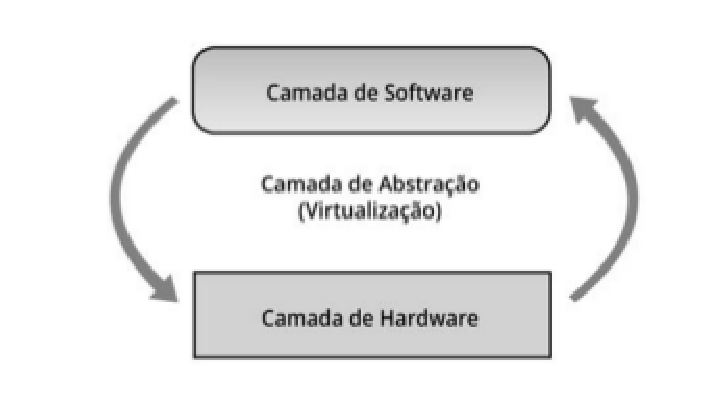
\includegraphics [keepaspectratio=true,scale=0.8]{figuras/virtualization_role.eps}
\caption{Responsabilidade da virtualização}
\cite{manoel}.
\label{virtualization_role}
\end{figure}

\section{Máquinas virtuais}
Uma máquina virtual é uma abstração em software de uma máquina física real. Destaca-se que é executada como uma aplicação padrão de usuário sobre um sistema operacional. A própria máquina virtual emula uma máquina física possuindo assim seus próprios discos e dispositivos \cite{mcewan}. Desse modo, umas das vantagens de máquinas virtuais reside na independência de uso do seu sistema operacional com relação ao sistema operacional da máquina física ao qual se encontra. Assim, em uma máquina física pode-se executar várias máquinas virtuais cada uma delas com sistemas operacionais diversos. A Figura \ref{arc_virtualization}, apresenta um exemplo de arquitetura de um ambiente virtualizado, utilizando um \textit{hypervisor} \textit{VMware}. Nela, observa-se que é na camada de virtualização que são providas as máquinas virtuais com seus respectivos sistemas operacionais e seus conjuntos de aplicações.% dividido em duas camadas: \textit{software} e \textit{hardware}. É na camada de software, mais espcificamente na camada de virtualização, através dos \textit{hypervisor}, que são providos as máquinas virtuais (hóspedes) com seus respectivos sistemais operacionais e \textit{hardwares} virtuais.  

\begin{figure}[!htb]
\centering
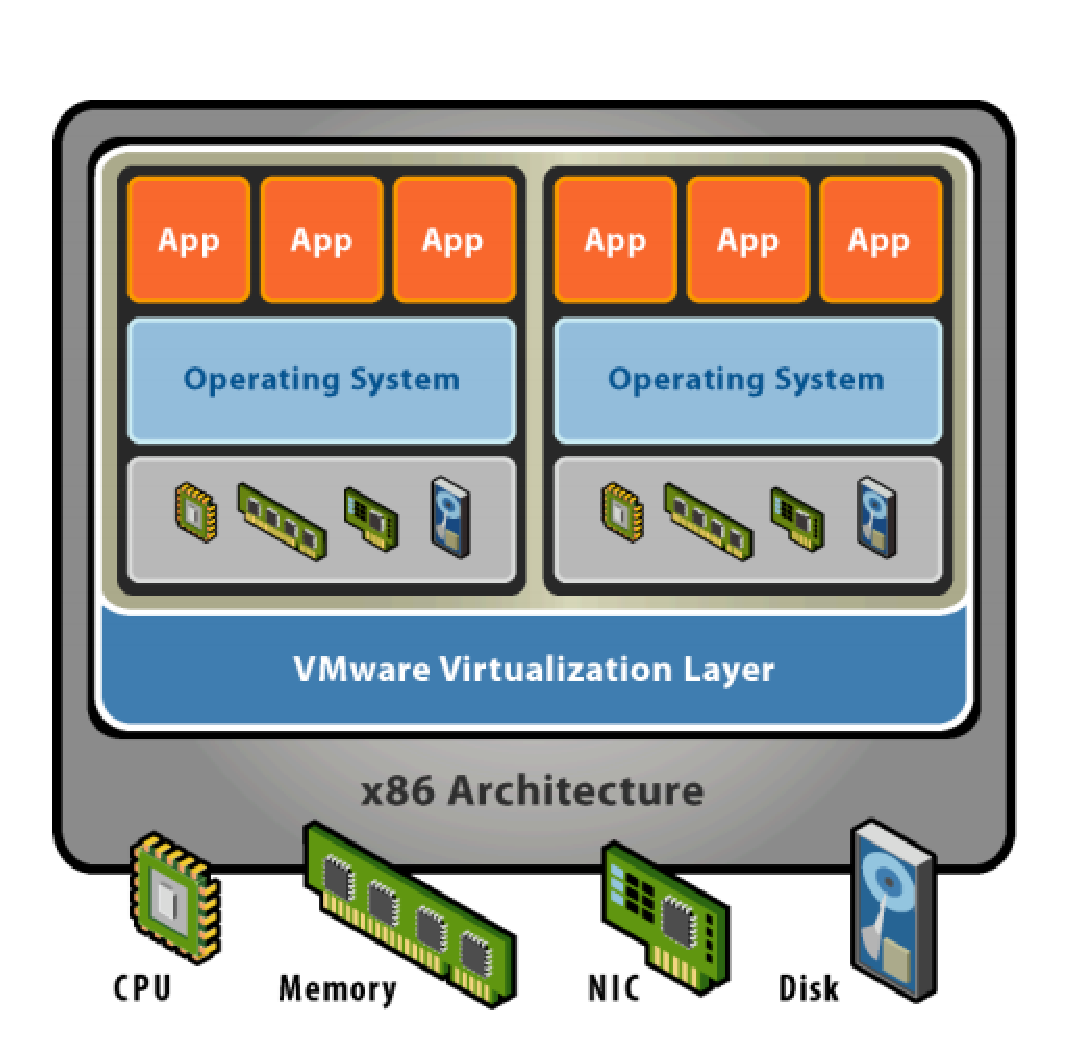
\includegraphics [keepaspectratio=true,scale=0.40]{figuras/virtualization_arc_2.eps}
\caption{Representação da implementação de um ambiente virtual}
\cite{vmware}.
\label{arc_virtualization}
\end{figure} 
 
\section{Monitor de Máquinas virtuais}
O \textit{hypervisor} (ou também conhecido como monitor de máquinas virtuais) é o software que possui mecanismos capazes de prover máquinas virtuais. Suas principais funções consistem no escalonamento de tarefas, gerência da memória e manutenção do estado da máquina virtual \cite{manoel}. Desse modo, atributos como desempenho e escalabilidade são determinantes para definir a qualidade dos serviços fornecidos por um \textit{hypervisor}. Algumas características são essenciais a um \textit{hypervisor}: segurança sobre os recursos virtualizados e agilidade na reconfiguração de recursos computacionais, sem interromper as operações do servidor de máquinas virtuais \cite{manoel}. Um \textit{hypervisor} pode ser classificado nos seguintes tipos:

\begin{itemize}
\item \textbf{Tipo I}(\textit{bare metal}, nativo ou supervisor): executa diretamente no hardware do servidor. Controla o hardware e o acesso do sistema operacional convidado(\textit{guest OS}. O papel do \textit{hypervisor} nativo é compartilhar os recursos de hardware entre as máquinas virtuais, de forma que cada uma delas imagina ter recursos exclusivos \cite{manoel}. Exemplos desse tipo incluem: \textit{VMware ESXi}, \textit{KVM}, \textit{Citrix XenServer}, e {Microsoft Hyper-V.}

\item \textbf{Tipo II}(\textit{hosted}): aplicação que fornece um ambiente de execução para outras aplicações. Executa sob um sistema operacional nativo como se fosse um processo deste. A camada de virtualização é composta por um sistema operacional hóspede e um hardware virtual, que são criados sobre os recursos de hardware oferecidos por meio do sistema operacional nativo \cite{manoel}.Exemplos desse tipo incluem: \textit{Oracle Virtual Box}, \textit{VMware, workstation.}
\end{itemize}

\section{Tipos de virtualização}
A virtualização pode ser realizada de diferentes maneiras, cada uma com seus prós e contras. Na prática, em arquiteturas x86, as opções de virtualização alteram o nível de privilégios padrões. As soluções baseadas em \textit{hypervisor} incluem a virtualização completa e a paravirtualização \cite{manoel}.

Antes de falar sobre os tipos de virtualização, é necessário que seja feita uma breve explicação sobre os níveis (ou anéis) de previlégio existentes em arquiteturas x86. Os anéis de privilégios, são níveis de permissões utilizados no gerenciamento de acessos ao \textit{hardware} de um sistema com arquitetura x86. Como apresentado na Figura \ref{rings}, são definidos 4 anéis de privilégio. Desse modo, aplicações a nível de usuário são geralmente executadas no Anel 3. Enquanto que sistemas operacionais, que precisam ter acesso direto à memória e ao \textit{hardware}, executam instruções privilegiadas no Anel 0 \cite{vmware}. 

\begin{figure}[!htb]
\centering
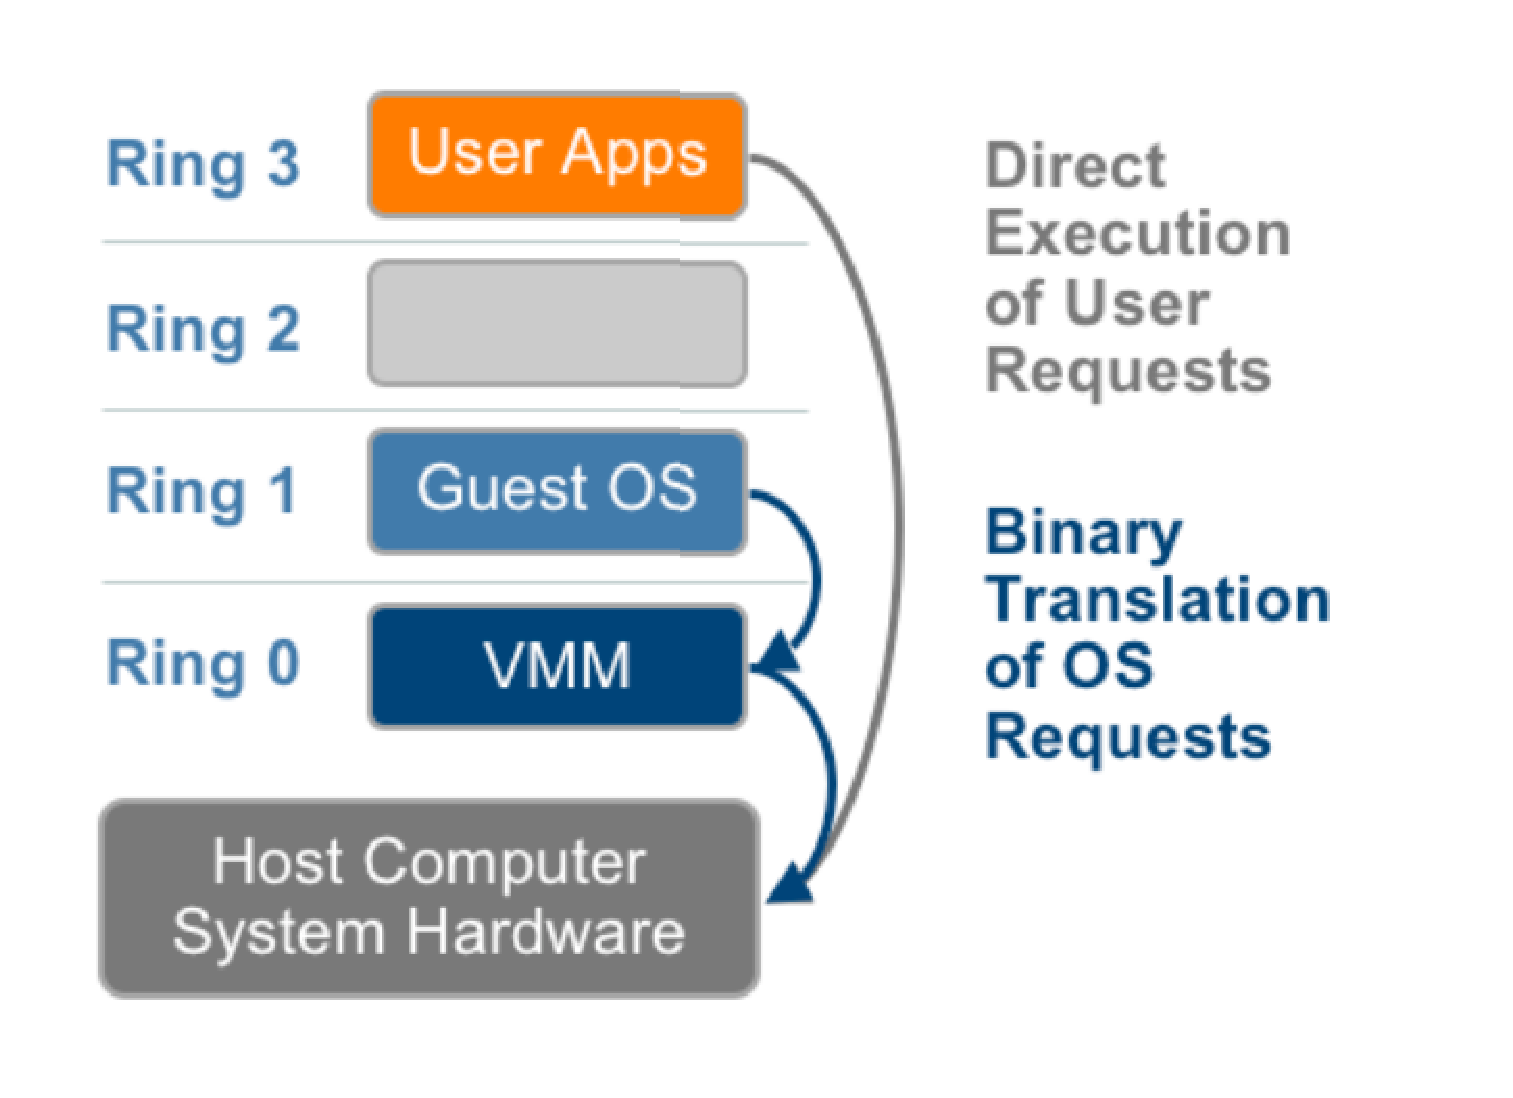
\includegraphics [keepaspectratio=true,scale=0.4]{figuras/rings.eps}
\caption{Representação da virtualização total}
\cite{vmware}.
\label{rings}
\end{figure}


Na virtualização total, uma estrutura completa de hardware é virtualizada, portanto o sistema operacional a ser virtualizado (sistema operacional hóspede) não precisa sofrer qualquer tipo de alteração, sendo esses um dos principais benefícios dessa técnica \cite{marcos}. Entretanto, o sistema virtualizado executa de forma mais lenta e o monitor de máquinas virtuais precisa implementar alternativas para que as operações privilegidas possam ser executadas em procesadores que não suportem a virtualização nativamente \cite{marcos}. Uma dessas alternativas é apresentada na Figura \ref{full_virtualization}, que mostra uma abordagem de virtualização total implementada pelo \textit{hypervisor} \textit{VMware}. Nessa abordagem, cada instrução sensível é substituída por uma chamada a uma rotina \textit{VMware} que a gerencia. Essa técnica é denominada de tradução binária. Já programas ou códigos que não possuem instruçõe sensíveis, são executados diretamente no \textit{hardware} \cite{tanembaum}.

Nota-se na Figura \ref{full_virtualization}, que o sistema operacional da máquina virtual (sistema operacional hóspede) está sendo executado em Anel 1, o que o impossibilitaria de executar instruções sensíveis. Entretanto, o \textit{hypervisor}, que está em Anel 0, intercepta as instruções sensíveis e as emula através da técnica de tradução binária, permitindo dessa forma, que o sistema operacional hóspede, mesmo estando em Anel 1, execute instruções sensíveis.

\begin{figure}[!htb]
\centering
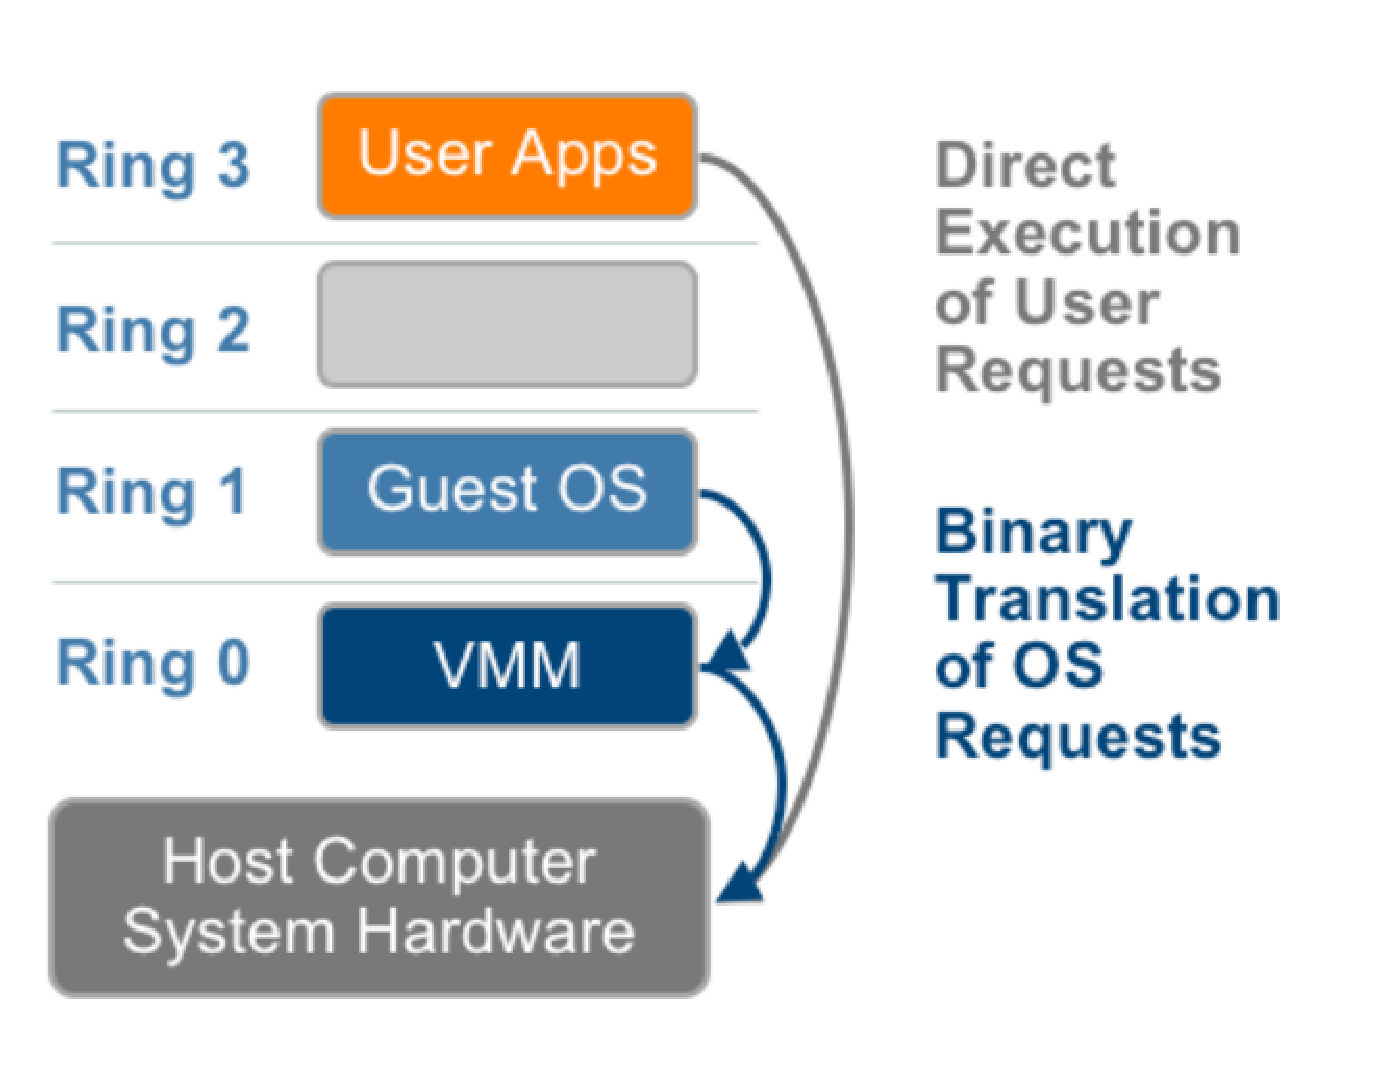
\includegraphics [keepaspectratio=true,scale=0.40]{figuras/full_virtualization_2.eps}
\caption{Representação da virtualização total}
\cite{vmware}.
\label{full_virtualization}
\end{figure}

Na paravirtualização, o sistema a ser virtualizado sofre modificações para que a interação com o monitor de máquinas virtuais seja mais eficiente, possibilitando que sistema operacional hóspede consiga acesar recursos do hardware diretamente. O acesso é monitorado pelo monitor de máquinas virtuais, que fornece ao sistema convidado recursos do sistema, tais como endereços de memória que podem ser utilizados e endereçamento em disco, por exemplo \cite{marcos}.

Dessa forma, como apresentado na Figura \ref{paravirtualization}, o sistema operacional hóspede é modificado de forma a executar, no lugar das instruções sensíveis, chamadas de \textit{hypervisor} \cite{tanembaum}. Destaca-se, que essa técnica faz com que o sistema operacional hóspede seja executado em Anel 0. A desvantagem dessa técnica de virtualização está relacionada, com a necessidade de se ter disponível o código fonte do sistema operacional hóspede, de modo que possa ser efutadas as modificações necessárias para que, o torne um sistema operacional paravirtualizado. Tornando difícil a aplicação dessa técnica em sistemas operacionais proprietários como o \textit{Windows} \cite{tanembaum}.
\begin{figure}[!htb]
\centering
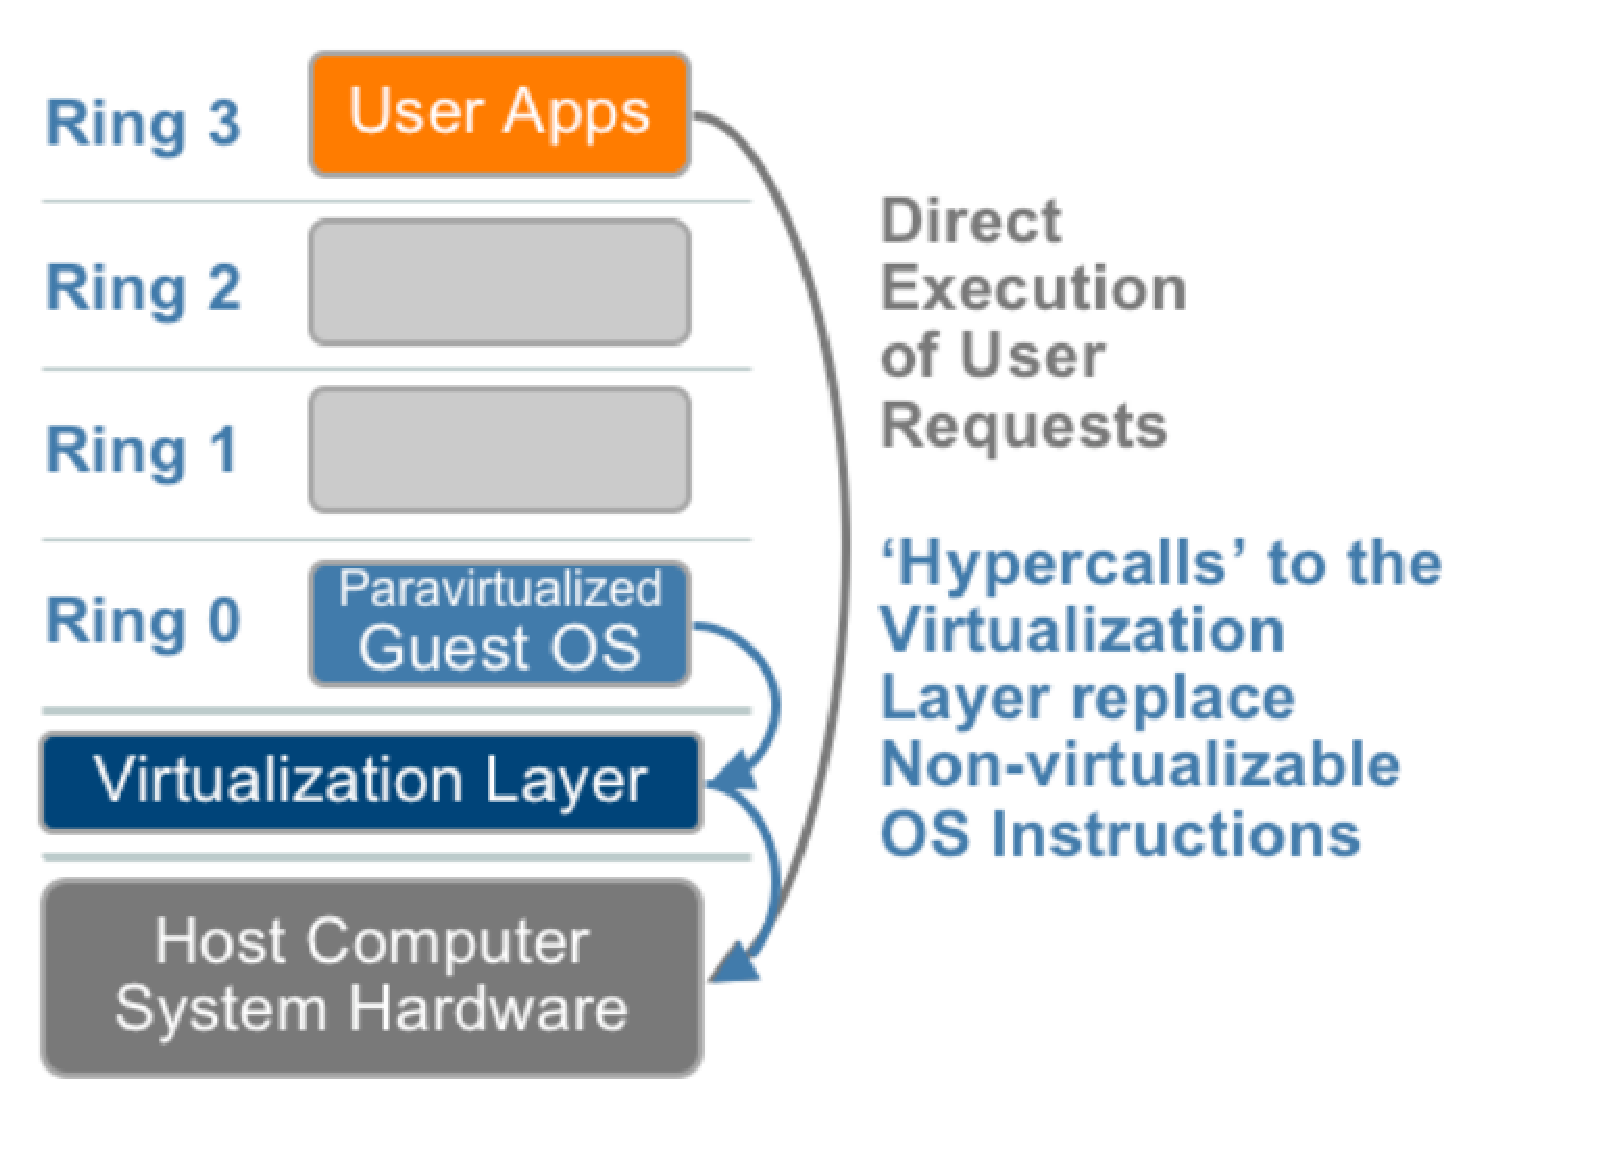
\includegraphics [keepaspectratio=true,scale=0.3]{figuras/paravirtualization2.eps}
\caption{Representação da paravirtualização}
\cite{vmware}.
\label{paravirtualization}
\end{figure}

\section{Ferramentas de Virtualização}
Nessa Seção serão abordadas algumas das ferramentas utilizadas para provimento de ambientes virtualizados: \textit{Xen} e\textit{KVM}. As ferramentas de virtualização basicamente são as plataformas responsáveis por prover a camada de virtualização ao qual serão disponibilizadas as máquinas virtuais.

O \textit{KVM} é uma solução de virtualização total voltada para arquiteturas x86. Possui suporte para tecnologias de virtualização \textit{Intel VT} e \textit{AMD-V}. Foi incorporado ao \textit{kernel} em janeiro de 2007, tornando-se assim um componente do \textit{Linux} sendo capaz de herdar as funcionalidade principais do mesmo \cite{redhatkvm,qumranet}.Pelo fato do KVM ter sido incorporado ao kernel do \textit{Linux}, o seu desenvolvimento passou a ter a colaboração ativa e o suporte da ampla comunidade do \textit{Linux} bem como de algumas fornecedoras da indústria do software tais como, Red Hat, AMD, HP, IBM, Intel, Novell, Siemens, SGI entre outros\cite {redhatkvm}.

O \textit{KVM} é implementado como um processo convencional do \textit{Linux}, de modo que cada \textit{CPU} virtual aparece como um processo regular. Proporcionando assim, ao \textit{KVM} os benefícios de todas as funcionalidades do \textit{kernel} do \textit{Linux}\cite{redhatkvm}. Como apresentado na Figura \ref{kvm_arc}, a emulação dos dispositivos e as operações de entrada e saída nos sistemas operacionais hóspedes, fica por conta de uma versão modificada do \textit{QEMU} \cite{redhatkvm,qumranet}. Neste, caso o \textit{KVM} intercepta eventos a niveis de sistema que precisam ser emulados, tais como leitura do disco ou o envio de um pacote pela rede, e invoca o \textit{QEMU} que emula a funcionalidade do \textit{hardware} requisitado \cite{rasmusson}. Por exemplo, a placa de rede virtual da máquina virtual que precisasse ser usada para algum envio de pacotes pela rede, teria esse tipo de funcionalidade emulada a partir da placa de rede física da máquina hospedeira. 

\begin{figure}[!htb]
\centering
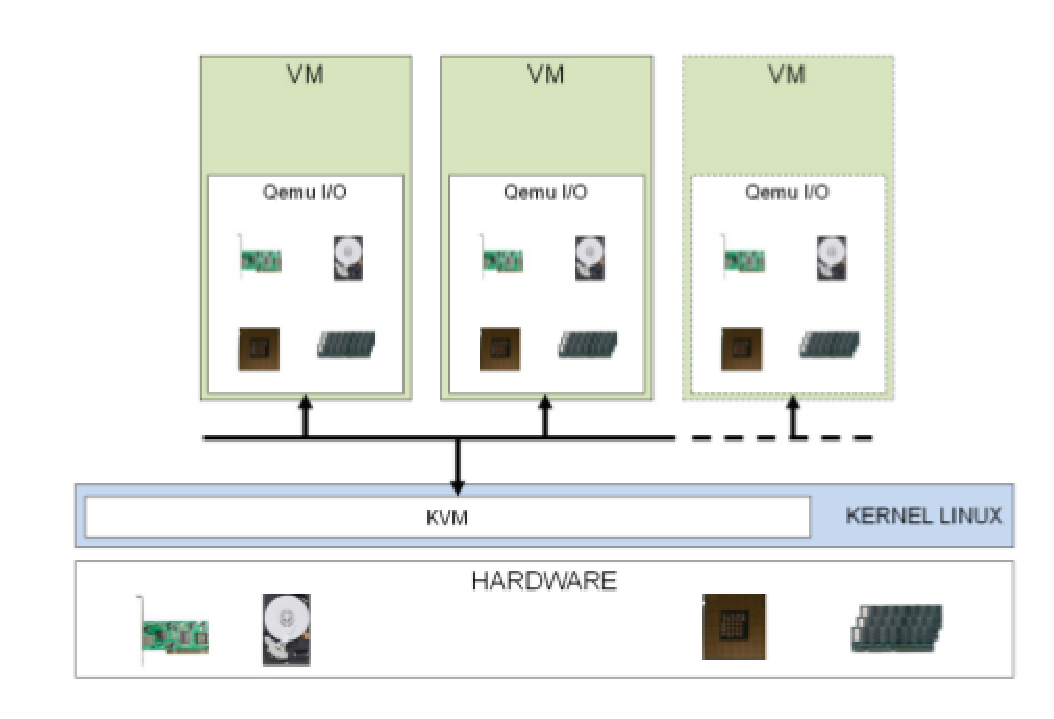
\includegraphics [keepaspectratio=true,scale=0.6]{figuras/kvm_arc.eps}
\caption{Arquitetura do KVM}
\cite{fabiano}.
\label{kvm_arc}
\end{figure}

Já o \textit{Xen} foi criado por Keir Fraser e Ian pratt como parte do projeto de pesquisa \textit{Xenoserver} pela \textit{Cambridge University}. Sendo que em 2002, teve seu código fonte aberto afim de promover melhorias no mesmo com a contribuição da comunidade de desenvolvedores. É um dos mais populares \textit{hypervisor} a implementar técnica de paravirtualização \cite{xen}. Desse modo é conhecido por possuir uma baixa perda de desempenho, se aproximando do desempenho nativo do servidor\cite{walters}. Isso é justificado pelo fato de que o sistema operacional das máquinas virtuais é modificado de modo que as chamadas privilegiadas são substituidas por chamadas diretas ao \textit{hypervisor}, ao contrário do que é feito com abordagens que utilizam emulação e tradução binária que acabam por focar no gerenciamento de chamadas previlegiadas \cite{redhatkvm}. 

\begin{figure}[h!]
\centering
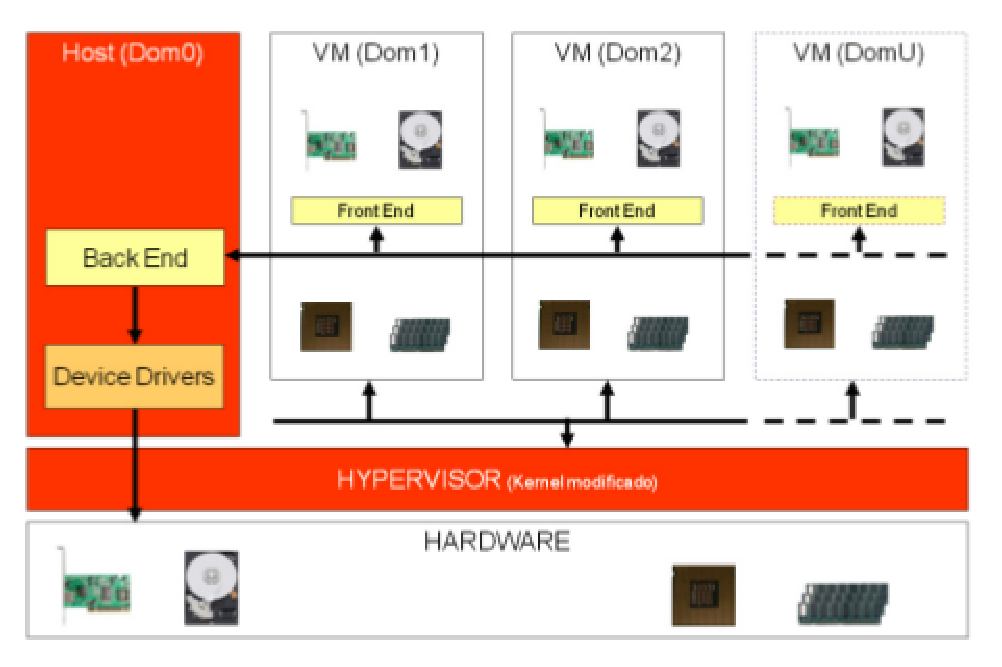
\includegraphics [keepaspectratio=true,scale=0.65]{figuras/xen_arquitecture.eps}
\caption{Arquitetura do XEN}
\cite{fabiano}.
\label{xen_arquitecture}
\end{figure}

A Figura \ref{xen_arquitecture} mostra que a arquitetura do \textit{Xen} é composta por dois componentes: o próprio \textit{hypervisor} \textit{Xen} e pelo domínio 0 (ou \textit{Dom0}). O \textit{hypervisor} \textit{Xen} é responsável por virtualização de memória e CPU, gerenciamento de energia e escalonamento das máquinas virtuais. Enquanto que o \textit{Dom0} é uma máquina virtual instanciada pelo próprio \textit{hypervisor} \textit{Xen} que possui acesso direto ao hardware, sendo responsável por prover \textit{drivers} dos dispostivos de E/S para máquinas virtuais \cite{redhatkvm}. As máquinas virtuais são conhecidas como \textit{DomU}(\textit{unprivileged domain}), sendo que as operações feitas por dispositivos de E/S são realizadas através da comunicação entre o processo \textit{front end}, existente no núcleo modificado das \textit{DomU}, e o processo \textit{back end}, existente no núcleo da \textit{Dom0} \cite{redhatkvm}.

Até aqui foram abordados os conceitos chaves que envolvem a virtualização bem como foram apresentadas duas ferramentas utilizadas no provimento da mesma (\textit{XEN} e \textit{KVM}). O que se percebe é que a virtualização traś consigo diversas possibilidades no que tange à tecnologias e ferramentas, cada qual com sua área de atuação, trazendo vantagens e desvantagens dependendo da necessidade de quem usa. Desse modo, a partir do que fora apresentado, este trabalho irá se concentrar na virtualização de servidores, utilizando a virtualização total através do \textit{hypervisor} \textit{KVM}.  

%Xen é um hipervisor do tipo 1 (ou baremetal) \textit{open source} para arquiteruas x86 que utiliza, por padrão a técnica de paravirtualização, \cite{clark}. Uma das maiores vantagens do uso do Xen como VMM na para-virtualização é o fato de que este apresenta um desempenho melhor do que os produtos de virtualização total, quando a máquina física hospedeira não tem instruções de hardware de suporte a virtualização \cite{eder}  

